\centering
\vspace{138mm}
\section*{\myul{Fluidstatik \& Hydrostatik}}

\begin{tikzpicture}[remember picture, overlay]

% --- ERSTE REIHE: Am Seitenursprung anfangen
\setlength{\rowheight}{100mm}

    % A1) Erste Kachel relativ zum Seitenursprung
    \setlength{\cellwidth}{86mm}
    \Tile{A1}{([xshift=10mm, yshift=-175mm]current page.north west)}{\cellwidth}{\rowheight}
        {
            \vspace{-\TileSep}
            \titlebf{Grenzfläche (Rotierender Zylinder)}\\ \vspace{-1mm}
            \begin{minipage}[t]{0.45\cellwidth-\TileSep}
                \centering
                \vspace{-2mm}
                \begin{equation*}
                    F_z = m\,\omega^2\,r = m\,\frac{v^2}{r}
                \end{equation*}%
                \vspace{0.25mm}
                \begin{equation*}
                    F_\text{G} = m\,g
                \end{equation*}
            \end{minipage}%
            \vline
            \begin{minipage}[t]{0.55\cellwidth-\TileSep}
                \centering
                \vspace{-2mm}
                \begin{equation*}
                    z(r) = H + \frac{\omega^2}{2\,g}\left(r^2 - \frac{1}{2}\,R^2\right)
                \end{equation*}
                \begin{equation*}
                    \tan\!\left(\alpha\right) = \frac{F_z}{F_\text{G}} = \frac{\omega^2\,r}{g}
                \end{equation*}%
                \vspace{-1mm}
            \end{minipage}%
            \vspace{2mm}
            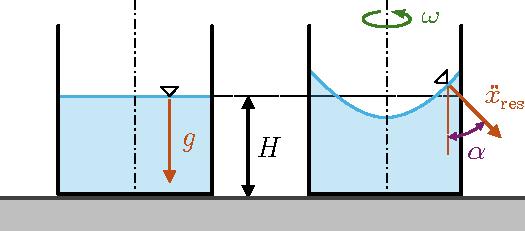
\includegraphics[width=65mm]{images/hydro-stat-dyn.pdf}
            \rule{\dimexpr\cellwidth-2\TileSep}{0.5pt} \\ \vspace{0.5mm}
            \titlebf{Hydrostatischer Auftrieb}\\ \vspace{2mm}
            \begin{minipage}{0.5\cellwidth-\TileSep}
                \centering
                \titlerm{Sinken / Schweben}\\ \vspace{-4mm}
                \begin{equation*}
                    F_\text{A} = \left(\rho_\text{F} - \rho_\text{K}\right)\,g\,V_\text{v}
                \end{equation*}%
                \vspace{-4mm}
            \end{minipage}%
            \vline
            \begin{minipage}{0.5\cellwidth-\TileSep}
                \centering
                \titlerm{Schwimmen}\\ \vspace{-4mm}
                \begin{equation*}
                    \rho_\text{F}\,g\,V_\text{v} = \rho_\text{K}\,g\,V_\text{K}
                \end{equation*}%
                \vspace{-4mm}
            \end{minipage}
            \begin{minipage}{0.42\cellwidth-\TileSep}
                \centering
                \scriptsize
                \begin{align*}
                    F_\text{A}    &= \text{Auftriebskraft} \\
                    \rho_\text{F} &= \text{Dichte (Fluid)} \\
                    \rho_\text{K} &= \text{Dichte (Körper)}
                \end{align*}
            \end{minipage}%
            \begin{minipage}{0.42\cellwidth-\TileSep}
                \centering
                \scriptsize
                \begin{align*}
                    g          &= \text{Erdbeschleunigung}   \\
                    V_\text{v} &= \text{Verdrängtes Volumen} \\
                    V_\text{K} &= \text{Volumen (Körper)}
                \end{align*}
            \end{minipage}
        }{0}{1}{0}{0}

    % B1) Zweite Kachel rechts anbauen
    \setlength{\cellwidth}{104mm}
    \Tile{B1}{(A1.north east)}{\cellwidth}{\rowheight}
        {
            \vspace{-\TileSep}
            \titlebf{Flüssigkeitssäule}\\ \vspace{2mm}
            \begin{minipage}{0.5\cellwidth-\TileSep}
                \centering
                \vspace{-2.5mm}
                \begin{equation*}
                    F_x = \frac{\rho\,g}{2}\left(y_2^2 - y_1^2\right)\,\text{d}z
                \end{equation*}
                \begin{equation*}
                    \text{d}F_x = \Delta p~\text{d}A_y
                \end{equation*}%
                \vspace{-3mm}
            \end{minipage}%
            \vline
            \begin{minipage}{0.5\cellwidth-\TileSep}
                \centering
                \vspace{-2.5mm}
                \begin{equation*}
                    F_y = \rho\,g\,\text{d}z\,\int_{x_1}^{x_2} y_\text{W}(x)\,\text{d}x
                \end{equation*}
                \begin{equation*}
                    \text{d}F_y = -\Delta p~\text{d}A_x
                \end{equation*}%
                \vspace{-3mm}
            \end{minipage}
            \begin{minipage}{0.65\cellwidth-\TileSep}
                \begin{equation*}
                    M_\text{A} = \rho\,g\,\text{d}z\left[\int_{x_1}^{x_2} x~y_\text{W}\!\left(x\right)\,\text{d}x - \frac{1}{3}\left(y_2^3 - y_1^3\right)\right]
                \end{equation*}
                \begin{equation*}
                    \left(
                    \begin{matrix}
                        x \\
                        y
                    \end{matrix}
                    \right)\times\left(
                    \begin{matrix}
                        \text{d}F_x \\
                        \text{d}F_y
                    \end{matrix}
                    \right)
                    = \text{d}M_\text{A} = x~\text{d}F_y - y~\text{d}F_x
                \end{equation*}
            \end{minipage}%
            \hspace{5mm}
            \begin{minipage}{0.28\cellwidth-\TileSep}
                \centering
                \vspace{2mm}
                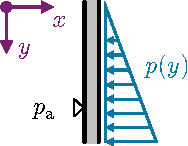
\includegraphics[width=19mm]{images/flüssigkeitssäule.pdf}\\ \vspace{-6mm}
                \begin{equation*}
                    \Delta p = p(y) - p_\text{a}
                \end{equation*}
            \end{minipage}%
            \vspace{2mm}
            \rule{\dimexpr\cellwidth-2\TileSep}{0.5pt} \\ \vspace{0.5mm}
            \titlebf{Atmosphäre}\\ \vspace{2mm}
            \begin{minipage}[t]{0.45\cellwidth-\TileSep}
                \centering
                \titlerm{Isotherm}\\ \vspace{-3mm}
                \begin{align*}
                    p(z)    &= p_0\,\exp\!\left(-\frac{\rho_0\,g}{p_0}\,z\right)    \\[0.75ex]
                    \rho(z) &= \rho_0\,\exp\!\left(-\frac{\rho_0\,g}{p_0}\,z\right) \\[2.5ex]
                    T(z)    &= T_0
                \end{align*}%
                \vspace{-1mm}
            \end{minipage}%
            \vline
            \begin{minipage}[t]{0.55\cellwidth-\TileSep}
                \centering
                \titlerm{Isentrop}\\ \vspace{-3mm}
                \begin{align*}
                    p(z)    &= p_0\left(1-\frac{\kappa-1}{\kappa}\,\frac{\rho_0\,g}{p_0}\,z\right)^{\frac{\kappa}{\kappa-1}}    \\
                    \rho(z) &= \rho_0\left(1-\frac{\kappa-1}{\kappa}\,\frac{\rho_0\,g}{p_0}\,z\right)^{\frac{\kappa}{\kappa-1}} \\[0.5ex]
                    T(z)    &= T_0\left(1-\frac{\kappa-1}{\kappa}\,\frac{\rho_0\,g}{p_0}\,z\right)
                \end{align*}%
                \vspace{-1mm}
            \end{minipage}
        }{0}{0}{0}{0}

\end{tikzpicture}